%----------------------------------------------------------------------------------------------------------------------------------------------------------%
\PassOptionsToPackage{sorting=none}{biblatex}
%----------------------------------------------------------------------------------------------------------------------------------------------------------%
\documentclass[fontsize=12pt,twoside=semi,openright,numbers=noenddot,parskip=half]{scrbook}
\usepackage{scrhack}\usepackage{mhotext}\usepackage{epigraph, geometry, graphicx, adjustbox, wrapfig, mathtools, booktabs, siunitx, setspace, subcaption, booktabs,multicol,dirtree,notoccite,xcolor,pifont,float}\usepackage[T1]{fontenc}\usepackage[UKenglish]{babel}\usepackage{gentium}
\usepackage{biblatex}[sorting=none,backend=biber,style=apa,citestyle=numeric-comp]\usepackage{pdfpages}\usepackage{enumitem}
\graphicspath{{./assets/}}\onehalfspacing
\addbibresource{references.bib}
%----------------------------------------------------------------------------------------------------------------------------------------------------------%
%\ihead{\leftmark}
%\chead{||Mar Roca Cugat||}
%\ohead{\ifstr{\leftmark}{\rightbotmark}{}{\rightbotmark}}
%\cfoot*{\pagemark}\
%----------------------------------------------------------------------------------------------------------------------------------------------------------%
\title{The Tale of a Bacteria Battle}
\subtitle{A study on \emph{Staphylococcus aureus}, its prevalence, clinical possibilities and our fighting tools}
\author{Mar Roca Cugat}
\date{Final draft}
%----------------------------------------------------------------------------------------------------------------------------------------------------------%
\begin{document}
\maketitle
\cleardoublepage
\renewcommand{\thepage}{\arabic{page}}
%----------------------------------------------------------------------------------------------------------------------------------------------------------%
\frontmatter
%----------------------------------------------------------------------------------------------------------------------------------------------------------%
\chapter{Acknowledgements}
\begin{center}
I would like to thank Margarita Martinez, professor at the \emph{Universitat de Girona}'s Microbiology Department, as well as Olga Sánchez, professor and researcher at the \emph{Universitat Autònoma de Barcelona}'s Department of Genetics and Microbiology for their help with certain aspects of this project. \newline
I would also like to acknowledge the magnificent work that the \LaTeX\ community does to give the scientific community an incredible piece of software with which to write, as well as to Mark Olson for making his \KOMAScript\ \TeX\ template open source, allowing anyone and everyone to use it and modify it for free. On that note, I'd also like to thank my friend, Gabriela, for helping me fix a weird issue with the bibliography system.\newline
But most importantly, I'd like to thank Núria Feliu, Imma Garcia and the rest of the science department for their monumental help which without this project could not have existed; as well as the subjects who volunteered to get their samples taken for this research.\newline
\end{center}
%----------------------------------------------------------------------------------------------------------------------------------------------------------%
\mainmatter\printindex\tableofcontents
%---------------------------------------------------------------------------------------------------------------------------------------------------------%
% > > > Introduction
%----------------------------------------------------------------------------------------------------------------------------------------------------------%
\chapter{Prologue}
%----------------------------------------------------------------------------------------------------------------------------------------------------------%
\epigraph{Good writing starts strong. Not with a cliché, not with a banality, but with a contentful observation that provokes curiosity.}{\textit{Stephen King}}
%----------------------------------------------------------------------------------------------------------------------------------------------------------%
A few years ago, in summer of 2021, I was accepted into a program at the Barcelona Autonomous University, aimed to divulge microbiology and biotechnology to a group of 50 biology-loving students. That's where I learned bacteria in detail, as well as how a microbiology/biotechnology lab functions. I fell in love with the discipline at first sight. I wondered how research in this field works, and so, I thought it was a good topic to develop for my Extended Essay.

\paragraph{}This Extended Essay has the objective of studying bibliographically the effects of \emph{Staphylococcus aureus} on the human body, as well as the ways humanity has developed to defeat it. Experimentally, it has one main objective, and several secondary ones: mainly, I want to find out the natural prevalence of Staphylococcus Aureus among my fellow schoolmates. Secondarily, I want to improve my lab etiquette and fluidity; to improve my protocol-making, how I follow them in the lab and how I deal with problems that may arise from them; to learn how to work with limited resources; and to practice my staining and microscope use. The research question I will follow is \emph``What is the prevalence of \emph{Staphylococcus aureus} in our school`` to which my hypothesis is ``About 30\%``. 

\paragraph{}This study requires taking samples from  human subjects. This is a one-off sampling process: the subjects are required only once. The results are then communicated to the subjects via e-mail or by being delivered a physical piece of paper. They are informed previously on the process they are going to go through, as well as the purpose of the experiment. Each subject must read and agree to two documents: an informed consent which explains everything about the experiment\footnote{See annex 1} and a GDPR notice which documents the use of their data as well as an expected timeline for data anonymisation and destruction\footnote{See annex 2}. All participants were screened to be over the age of 16, in order to ease the process and require no previous authorisation by parental figures on the data collection. The experimentation followed has no effect on the subjects\cite{WhatGDPREU2018}.
\paragraph{}Since bacteria were used, some aspects of the experiment must be clarified and discussed. Previously to starting the experiment, I read profusely the WHO's Laboratory Biosafety Manual and Associated Monographs (4Th Edition)\cite{worldhealthorganizationLaboratoryBiosafetyManual2020} in order to find ways to mitigate any possible risk. During the experimental phases, there were no accidents or incidents. All plates were accounted for and controlled closely. No person other than me was allowed to come in contact with a plate that had been cultivated or with any used but not disinfected auxiliary material. The cultivated plates were considered Biosecurity Level 2. All possibly infected material was disposed of taking into account the risks that the bacteria in question posed, using fresh bleach.
\paragraph{}Before starting the experimentation, and following the guidelines dictated by the IBO about the EE, I had a talk with my coordinator in order to solidify the fact that there was no alternative to taking cutaneous samples from human beings, as well as a discussion on bacteria and the risks that this experiment implies.

% > > > Introduction
%----------------------------------------------------------------------------------------------------------------------------------------------------------%
\chapter{Theoretical context}
%----------------------------------------------------------------------------------------------------------------------------------------------------------%
\epigraph{Each source that I read, I would look through the bibliography and the footnotes, and use that as a map for the next thing I would read.}{\textit{Alexander Chee}}
%----------------------------------------------------------------------------------------------------------------------------------------------------------%
\section{Bacteria and bacterial infections}
\paragraph{Bacteria} are prokaryotic organisms, generally single-celled, which are part of the Monera kingdom. Their sizes range from between 30\textmu m and 100\textmu m and are ubiquitous\footnote{Ubiquitous: found everywhere} organisms. This form of life is believed to be the first one to have ever appeared on Earth, as well as the one responsible for the oxygen-rich atmosphere the Earth currently has. Some species are hard to culture in a laboratory environment, but generally, those that can be cultured in a controlled environment are grown in agar plates\cite{murrayMicrobiologiaMedica2013}. \newline
\paragraph{Pathogenic bacteria} are bacteria that have the ability to cause disease\footnote{A disease is a particular abnormal condition that negatively affects the structure or function of all or part of an organism, and that is not immediately due to any external injury\cite{DorlandsMedicalDictionary2010}.} These are not the most common type of bacteria, as the majority of them are either harmless or beneficial to the human body through symbiosis, such as the bacteria that help with digestion in the stomach\cite{murrayMicrobiologiaMedica2013}.
%----------------------------------------------------------------------------------------------------------------------------------------------------------%
\section{The enemy: \emph{Staphylococcus aureus}}
\paragraph{}\emph{Staphylococcus aureus} (also known as Staph) is a GRAM-positive bacterium, usually not pathogenic. It can, in some cases, cause extremely dangerous infections. Some of its distinctive characteristics include a very thick glycopeptide wall, which allows it to withstand extreme temperatures and osmotic pressures, rendering most classic methods of food conservation\footnote{Cooking, smoking, freezing, salting...} useless against it; a protein A capsid, which binds to most eukaryote cells; as well as thermoresistant enterotoxins. It's a bacterium that can resist many environments, and can found on human skin, mucotic surfaces, as well as in certain foods such as ham, eggs, and poultry\cite{nutritionBAMChapter122020}.\newpage
\begin{wrapfigure}{r}{0.5\textwidth}\begin{center}\includegraphics[width=0.48\textwidth]{staph_parts.png}\end{center}\caption{Parts of \emph{Staphylococcus aureus}\cite{kongCommunityAssociatedMethicillinResistantStaphylococcus2016}.}\end{wrapfigure}
\paragraph{}Staphylococcus aureus has three main parts to its virulence: its cell wall, its membrane-bound factors and its secreted factors. Staph's cell wall is made up of three parts. From the inside out they are: a plasma membrane, a peptidoglycan layer and a capsule\cite{kongCommunityAssociatedMethicillinResistantStaphylococcus2016}.
The membrane includes a semipermeable lipid bi-layer, which regulates the transport of materials entering and exiting the cell. Integrated inside it are a type of integral protein called penicillin-binding protein (PBP), along with proteins dedicated to powered transport. We are only interested in PBPs. Even though the name
 implies PBPs are only sensible to penicillin, the name actually came to be this way because of their discovery. These proteins are sensitive to the \textbeta-lactam groups in antibiotics. Variations in them may lead to antibiotic-resistant strains, such as MRSA (\emph{Methicillin-Resistant \emph{Staphylococcus aureus}}), result of a mutation in this protein called PBPA2\cite{kongTargetingStaphylococcusAureus2016}. \newline
\emph{Staphylococcus aureus}, like all other members of the \emph{Staphylococcus} family, has a very thick peptidoglycan layer. This grants them protection from extreme temperatures and high osmotic pressures. Since little to no other bacteria can survive in the conditions that Staph can, it starts reproducing without the limit that would be imposed by having other bacteria competing for the same resources\cite{clareticomaResistenciaAntibioticaPoblacions2004}.
%----------------------------------------------------------------------------------------------------------------------------------------------------------%
\section{The enemy's attacks}
\paragraph{}\emph{Staphylococcus aureus} is a species that can cause a handful of different diseases, ranging from, most frequently, skin and respiratory tract infections to infective endocarditis, toxic shock syndrome or osteomyelitis\cite{cheungPathogenicityVirulenceStaphylococcus2021}. Several variations of this pathogen exist, with increasing levels of antibiotic resistance: MSSA (\emph{Methicillin-Sensitive Staphylococcus aureus}), having no resistance; MRSA (\emph{Methicillin-Resistant Staphylococcus aureus}); and VRSA (\emph{Vancomycin-Resistant Staphylococcus aureus}), the   latter for which no antibiotic concoction that can eradicate the infection is known, and the patients have to use experimental treatments. VISA (\emph{Vancomycin-intermediate Staphylococcus aureus}) is a variation that has medium resistance to vancomycin, being an intermediate step between MRSA and VRSA. Studies have discovered that this genetic factor has been developed by different lineages separately, indicating that there is not a common ancestor of MRSA strains\cite{zhouReviewNanosystemsEffective2018}.
\paragraph{}\emph{Staphylococcus aureus} contains an important quantity of \textbf{toxins}, compounds that grant \emph{Staph} most of its pathogenicity. Many of its virulence factors can be described as such. Toxins are usually defined as poisonous substances, which, in our case, means that they have the capacity to mess with the host body directly, without need of a mediating entity. Staph has several kinds of toxin in its arsenal: membrane-damaging toxins (which can be receptor-mediated or not), receptor-interfering toxins (which do not damage the membrane), enzymes, and pathway blockers\cite{kongTargetingStaphylococcusAureus2016}.\newline
%----------------------------------------------------------------------------------------------------------------------------------------------------------%
\section{Our weapons}
\paragraph{} The tools we have at our disposal to fight off this infection fall into two main categories: chemical factors and biological factors.
\paragraph{} The chemical factors are drugs, and they depend both in quantity and type on the variation a particular case falls in. It is \textbf{extremely important} to find out the level of antibiotic resistance that a specific infection has before administering any antibiotic, as this treatment course will cause side effects such as killing gut bacteria, diminishing defence system capabilities, and increasing the possibility to develop yet more resistant infections. Generally, a large-spectrum antibiotic has an adequate risk-to-benefits ratio of causing the previously mentioned side effects, so they may be used before switching to a more specific (and in some cases even more violent) treatment.
\paragraph{}\begin{wrapfigure}{r}{0.35\textwidth}\begin{center}\includegraphics[width=0.30\textwidth]{assets/beta-lactam.png}\end{center}\caption{Organic chemistry structure of penicillin (top) and cephalosporin (bottom). The \textbeta-lactam ring is indicated in red. Source: \cite{fvasconcellosSkeletalFormulaeBasic}}\end{wrapfigure}Starting with the treatment to the least resistant strains of \emph{Staphylococcus aureus}, a \textbeta-lactam antibiotic (such as methicillin, oxacillin, cloxacillin and penicillin) is the weapon of choice to fight against an MSSA infection. This is because this specific chemical part (just a \textbeta-lactam ring does nothing by itself) has the ability to inhibit cell wall biosynthesis on the bacterial intruder's body. But once the \textbeta-lactam ring is cut by an enzyme secreted by the bacteria itself, this type of antibiotic suddenly loses effect against them.
\paragraph{}That's where vancomycin comes in. It is a type of glycopeptide antibiotic, just like \textbeta-lactam, and works by blocking the construction of a cell wall, as all of its type do.
\begin{wrapfigure}{l}{0.35\textwidth}\begin{center}\includegraphics[width=0.30\textwidth]{assets/vancomycin.png}\end{center}\caption{Organic chemistry structure of vancomycin. Source: \cite{bartvl71ChemicalStructureVancomycin}}\vspace{0.15\linewidth}\end{wrapfigure}This treatment is very invasive and only indicated for the treatment of extremely serious, life-threatening infections by Gram-positive bacteria that have shown to be unresponsive to other antibiotics.It can be taken as a pill or as an injectable fluid, the latter form proving to be much more effective than the former. This treatment is incompatible with aminoglycosides, a type of antibiotic that inhibits protein synthesis, as it can lead to nephrotoxicity and ototoxicity. Vancomycin can induce  internal bleeding, with petechial haemorrhages on the tongue and bruises on most of the body of the patient. Unfortunately, even with use of vancomycin, \emph{Staphylococcus aureus} can develop resistance. In this case, no other option than using a biological factor is left.
\newpage\paragraph{}The biological factor is a bacteriophage, called P68. It comes from the \emph{Caudovirales} order, which means that it is a bacteriophage with tail.  This treatment is still in testing, but it appears to be effective and lead to low adverse results. If possible, it would be preferable to use bacteriophage therapy (shortened to phage therapy) instead of going for antibiotics, as it can lead to less side effects than antibiotics, as it only attacks a specific bacterium. This means that the infection has to be pinpointed with extreme accuracy. The use of this treatment also negates the risk of bacteria developing antibiotic resistance. It is, however, unclear whether the bacteriophage could mutate into a dangerous strain. This therapy is in clinical research, and may be available soon.\cite{zhouReviewNanosystemsEffective2018}\cite{eskenaziCombinationPreadaptedBacteriophage2022}.
\newpage{}\begin{wrapfigure}{r}{0.35\textwidth}\begin{center}\includegraphics[width=0.30\textwidth]{assets/staph_side.png}\end{center}\caption{External structure of P-68, graphed using AlphaFold. Own source.}\end{wrapfigure}Bacteriophages work in an interesting manner. They work by detecting one very specific bacteria, just like any other virus does with the type of cell they evolved for, then bind to it and inject their genetic material, which then in turn the bacteria considers as its own, inserts it into its own genetic sequence and starts producing the proteins the virus requires, but it doesn't eject them. Once the bacteria is full of phages, a special lytic compound is released which bursts the cell membrane in such a way that it resembles an explosion, but instead of heating up everything in a radius, spreads millions more of bacteriophages, which then bind to other bacteria and the cycle repeats until there's no more bacteria left. The fight from the bacteria point of view consists mostly on trying to outnumber and outreproduce the phages in order to have a chance of survival, even if minimal. There is no known bacteria that shows resistance to phages. That is probably because, unlike the chemical factors, phages can evolve and improve with each generation thanks to natural selection\cite{hrebikStructureGenomeEjection2019a}.

% > > > Experimental, round 1
%----------------------------------------------------------------------------------------------------------------------------------------------------------%
\chapter{Physical experimentation}
\epigraph{A scientist in his laboratory is not a mere technician: he is also a child confronting natural phenomena that impress him as though they were fairy tales.}{\textit{Marie Curie}}
%----------------------------------------------------------------------------------------------------------------------------------------------------------%
\section{Description}
\paragraph{}This experiment looks at finding out the prevalence of \emph{Staphylococcus aureus} in a sample of students from the school. The process used involves extracting a sample from underneath a subject's nails by swabbing, cultivating that sample and then observing the results of said culture to determine the presence or not of \emph{Staphylococcus aureus} as part of the subject's resident bacterial flora. Each iteration of the process took less than two minutes to complete. However, all the safety measures and actions taken need more time to be taken care of properly.
%----------------------------------------------------------------------------------------------------------------------------------------------------------%
\section{Protocol followed}
\paragraph{}The protocol followed was designed based on a similar protocol used in the many university laboratories\cite{olearyPracticalHandbookMicrobiology1989}, modified to fit the needs of this research paper, and peer-reviewed by Olga Sánchez, and uploaded to the Protocols.io platform, to make it easier to follow the days of that the experiment took place in. This protocol underwent 10 different revisions\cite{rocacugatStaphilococcusAureusSampling2022a}. It can also be read below:\newline\begin{wrapfigure}{r}{0.4\textwidth}\begin{center}\includegraphics[width=0.38\textwidth]{sampling.JPG}\end{center}\caption{Transferring a sample to the agar plate}\end{wrapfigure}
\begin{enumerate}[label=\arabic*)]
\item Prepare yourself for the experimentation: wash your hands, put on gloves, put on the lab coat, mask and goggles. Wash your hands again (gloves still on). Set up the work area; the Bunsen burner should be turned on in such a way that it can cover an acceptable surface to work. Turn it on and wash your hands again.
\item Divide each Petri dish between 2 parts. A guide should be used for this part. Get your subject to wash their hands. Observe their hands. If they are extremely short, it may be worth it to take the sample nasally.
\item Note down their information, crack open a sterile swab, dip it in Ringer solution and swab away at under their nails or nose. Then, populate the dish with this sample.
\item Incubate for 32-48h and observe the results.
\item Observe the bacteria under a microscope after GRAM tinction.
\end{enumerate}\newpage
%----------------------------------------------------------------------------------------------------------------------------------------------------------%
\section{Bill of materials}
\paragraph{}The materials used, as well as the quantities used can be found in the following table. On the left, laboratory equipment and, on the right, reagents, tinction agents, and consumables used:
\begin{center}\begin{figure}[H]\centering\includegraphics[width=0.90\textwidth]{BOM-1.png}\end{figure}\end{center}
%----------------------------------------------------------------------------------------------------------------------------------------------------------%
\section{Biosecurity and risk mitigation}
\paragraph{}Staph is considered a Biosecurity Level (BSL) 2 pathogenic bacteria\cite{cheungPathogenicityVirulenceStaphylococcus2021}. This means that the it is associated with a human disease that can pose a moderate human health hazard. In a laboratory where BSL-2 pathogens are handled, regular lab rules should be followed (mechanical pipetting only, hand washing, prohibition of the consumption of food and drinks in the lab, proper PPE use...), as well as avoiding splashes or aerosols, adhering biohazard warning signs present on all material used, as well as proper surface and material disinfection via the use of autoclave or proper alternative decontamination method\cite{worldhealthorganizationLaboratoryBiosafetyManual2020}.\newline
The risks associated with this bacteria were assessed following the protocol designated by the World Health Organisation, and proper security measures were followed at all times when handling biohazardous material. No incidents occurred during the research part of this project, and the protocol defined previous to the start was followed extremely closely. While the laboratory used may not be the most ideal type of laboratory for this type of research, it was certainly adequate enough to perform a research project like this one, especially after the temporary signage that was temporarily installed.
%----------------------------------------------------------------------------------------------------------------------------------------------------------%
\section{Results and analysis}
The results obtained can be found in the following raw data table:
\begin{center}\begin{figure}[H]\centering\includegraphics[width=0.90\textwidth]{RES-1.jpg}\end{figure}\end{center}\vspace{-4cm}
The data was then recounted and graphed into the following pie chart:
\begin{center}\begin{figure}[H]\centering\begin{subfigure}[b]{0.4\linewidth}\includegraphics[width=\linewidth]{Data.png}\caption{Counts of the result cases.}\end{subfigure}\begin{subfigure}[b]{0.4\linewidth}\includegraphics[width=\linewidth]{Pie.png}\caption{Pie graph of the result cases.}\end{subfigure}\caption{Data processed from results}\end{figure}\end{center}\vspace{-1.5em}
As we can see, almost 50\% of the samples taken tested positive for \emph{Staphylococcus aureus}, compared to the expected 30\%\cite{StaphylococcusAureusHealthcare2020}. We can, however, see in the UK's Public Health bactaeremia data that Staph infections have been on the rise lately, so it may not be a case of wrong data\cite{englandMSSABacteraemiaAnnual2021}. On top of that, both of my advisers, Olga and Margarita, have also found themselves getting more prevalence than usual of this bacteria, and are finding cases that were once negative but turned positive in the last few years. Most of these results were not only confirmed by the highly-specific detection of the MSA plate, but also by doing morphological observation, both of the colonies and microscopically.\begin{figure}[H]\centering\begin{subfigure}[b]{0.4\linewidth}\includegraphics[width=\linewidth]{microscope.JPG}\caption{\emph{Staphylococcus aureus} as seen below the microscope. x4000, GRAM tinction}\end{subfigure}\begin{subfigure}[b]{0.4\linewidth}\includegraphics[width=\linewidth]{colonies.JPG}\caption{Colonies of \emph{Staphylococcus aureus} seen under a magnifying glass}\end{subfigure}\caption{Photographies of the results, as collected from my own experimentation (own data).}\end{figure}\paragraph{}There may be several reasons for the infection rate and thus natural prevalence to be increasing. One of them could be that since antibiotic abuse is growing with each passing year, the usual resident microbiota is getting killed, leaving more resources for Staph to thrive in that environment. To confirm this theory we will look at the infection rates of a country that is facing extreme antibiotic abuse (the United States of America) and compare it to another that is controlling their antibiotics a bit better (the United Kingdom). They have seen a 210\% increase in \emph{Staphylococcus aureus} cases since 2006. However, superfluous antibiotic prescriptions have increased by barely 1\%\cite{baggsEstimatingNationalTrends2016}. In the United Kingdom, they have seen a 160\% increase in \emph{Staphylococcus aureus} infections\cite{englandMSSABacteraemiaAnnual2021}, and their superfluous antibiotic prescriptions have gone down by 20\%. While this seems like very little data to extract conclusions from, it is clear that there may be a correlation between these two factors.
\paragraph{}The other could be climate change. An increase of ambient temperatures could mean a better breeding ground for this specific species and thus leading to a higher-than-usual prevalence. \emph{Staphylococcus aureus}' optimal breeding temperature is between 35\si{\celsius} and 37\si{\celsius}. The global average temperature has increased by 1,1\si{\celsius}\cite{gmsGMSAnnualGlobal2016} in the last 120 years. And \emph{Staphylococcus aureus} has a specific temperature growth curve, just like any other bacteria:\begin{figure}[H]\centering\begin{subfigure}[b]{0.4\linewidth}\includegraphics[width=\linewidth]{tempcurve.png}\caption{\emph{Staphylococcus aureus} growth curve by temperature\cite{FigEffectTemperature2022}}\end{subfigure}\begin{subfigure}[b]{0.4\linewidth}\includegraphics[width=\linewidth]{warm.png}\caption{Global warming plotted by the year\cite{GlobalWarming2010}}\end{subfigure}\caption{Graphs relating the temperature of growth of \emph{Staphylococcus aureus} and the increase of temperature of the Earth.}\end{figure}So, this correlation may not be completely incorrect, and in fact some scientists warn about an increased number of infectious diseases resurging due to climate change. One only data point is not enough significant data, so further study is needed on this front.


% > > > Experimental, round 2
%----------------------------------------------------------------------------------------------------------------------------------------------------------%
\chapter{Computational experimentation}
%----------------------------------------------------------------------------------------------------------------------------------------------------------%
\epigraph{Remember that all models are wrong; the practical question is how wrong do they have to be to not be useful.}{\textit{Norman Richard Draper}}
%----------------------------------------------------------------------------------------------------------------------------------------------------------%
\section{Description}
\paragraph{}This second experiment looks at computing the shape of a \emph{Staphylococcus aureus} P-68 bacteriophage starting from its DNA sequence. This will analyse the process of protein translation, as well as looking at the process of using AlphaFold\cite{jumperHighlyAccurateProtein2021}. To compute the secondary, tertiary and quaternary structures of the proteic parts of the virus we will use the Google CoLaboratory version of AlphaFold\cite{GoogleColaboratoryAlpha1970}, as it allows for far more computer power than available on a simple laptop.
%----------------------------------------------------------------------------------------------------------------------------------------------------------%
\section{Protocol followed}
The protocol followed is very simple, as AlphaFold, the Artificial Intelligence model used, does the hardest part of the work for us: calculating the secondary, tertiary and quaternary structures.
\begin{enumerate}[label=\arabic*)]
\item Convert the DNA sequence of one of the proteins to an mRNA sequence, by taking into account the fact that there's base complementarity.
\item Convert the mRNA sequence to an amino acid sequence of the proteins by using the genetic universal code table.
\item Feed the amino acid sequences to AlphaFold, and obtain the PDB models for each protein.
\item Assemble the bacteriophage.
\item Print, polish and paint a 3D physical model of the bacteriophage to illustrate better how it functions.
\end{enumerate}
The AlphaFold Jupiter notebook\cite{GoogleColaboratoryAlpha-} used is optimized for use with the NVIDIA Tesla T4 computing engine GPU, an extremely powerful graphics card, like the ones used in computers to render extremely detailed polygons in video games or 3D animations. That's the one I used when folding\footnote{Folding a protein: calculating, by using the theoretical intermolecular forces, the shape of the protein} the proteins. The genomic sequence used is NC\_004679.1, which leads to the PDB structure 6Q3G.
%----------------------------------------------------------------------------------------------------------------------------------------------------------%
\section{Results and analysis}
The gene codified for a total of 22 separate proteins. After BLASTing\footnote{BLAST: digital service that takes a sequence of DNA in the FASTA format and attempts to find the organism and/or protein that it codifies} all of them, I got the following list:
\begin{center}\begin{figure}[H]\centering\includegraphics[width=0.90\textwidth]{AF3.png}\end{figure}\end{center}
Which then assembled into the following figure:
\begin{center}\begin{figure}[H]\centering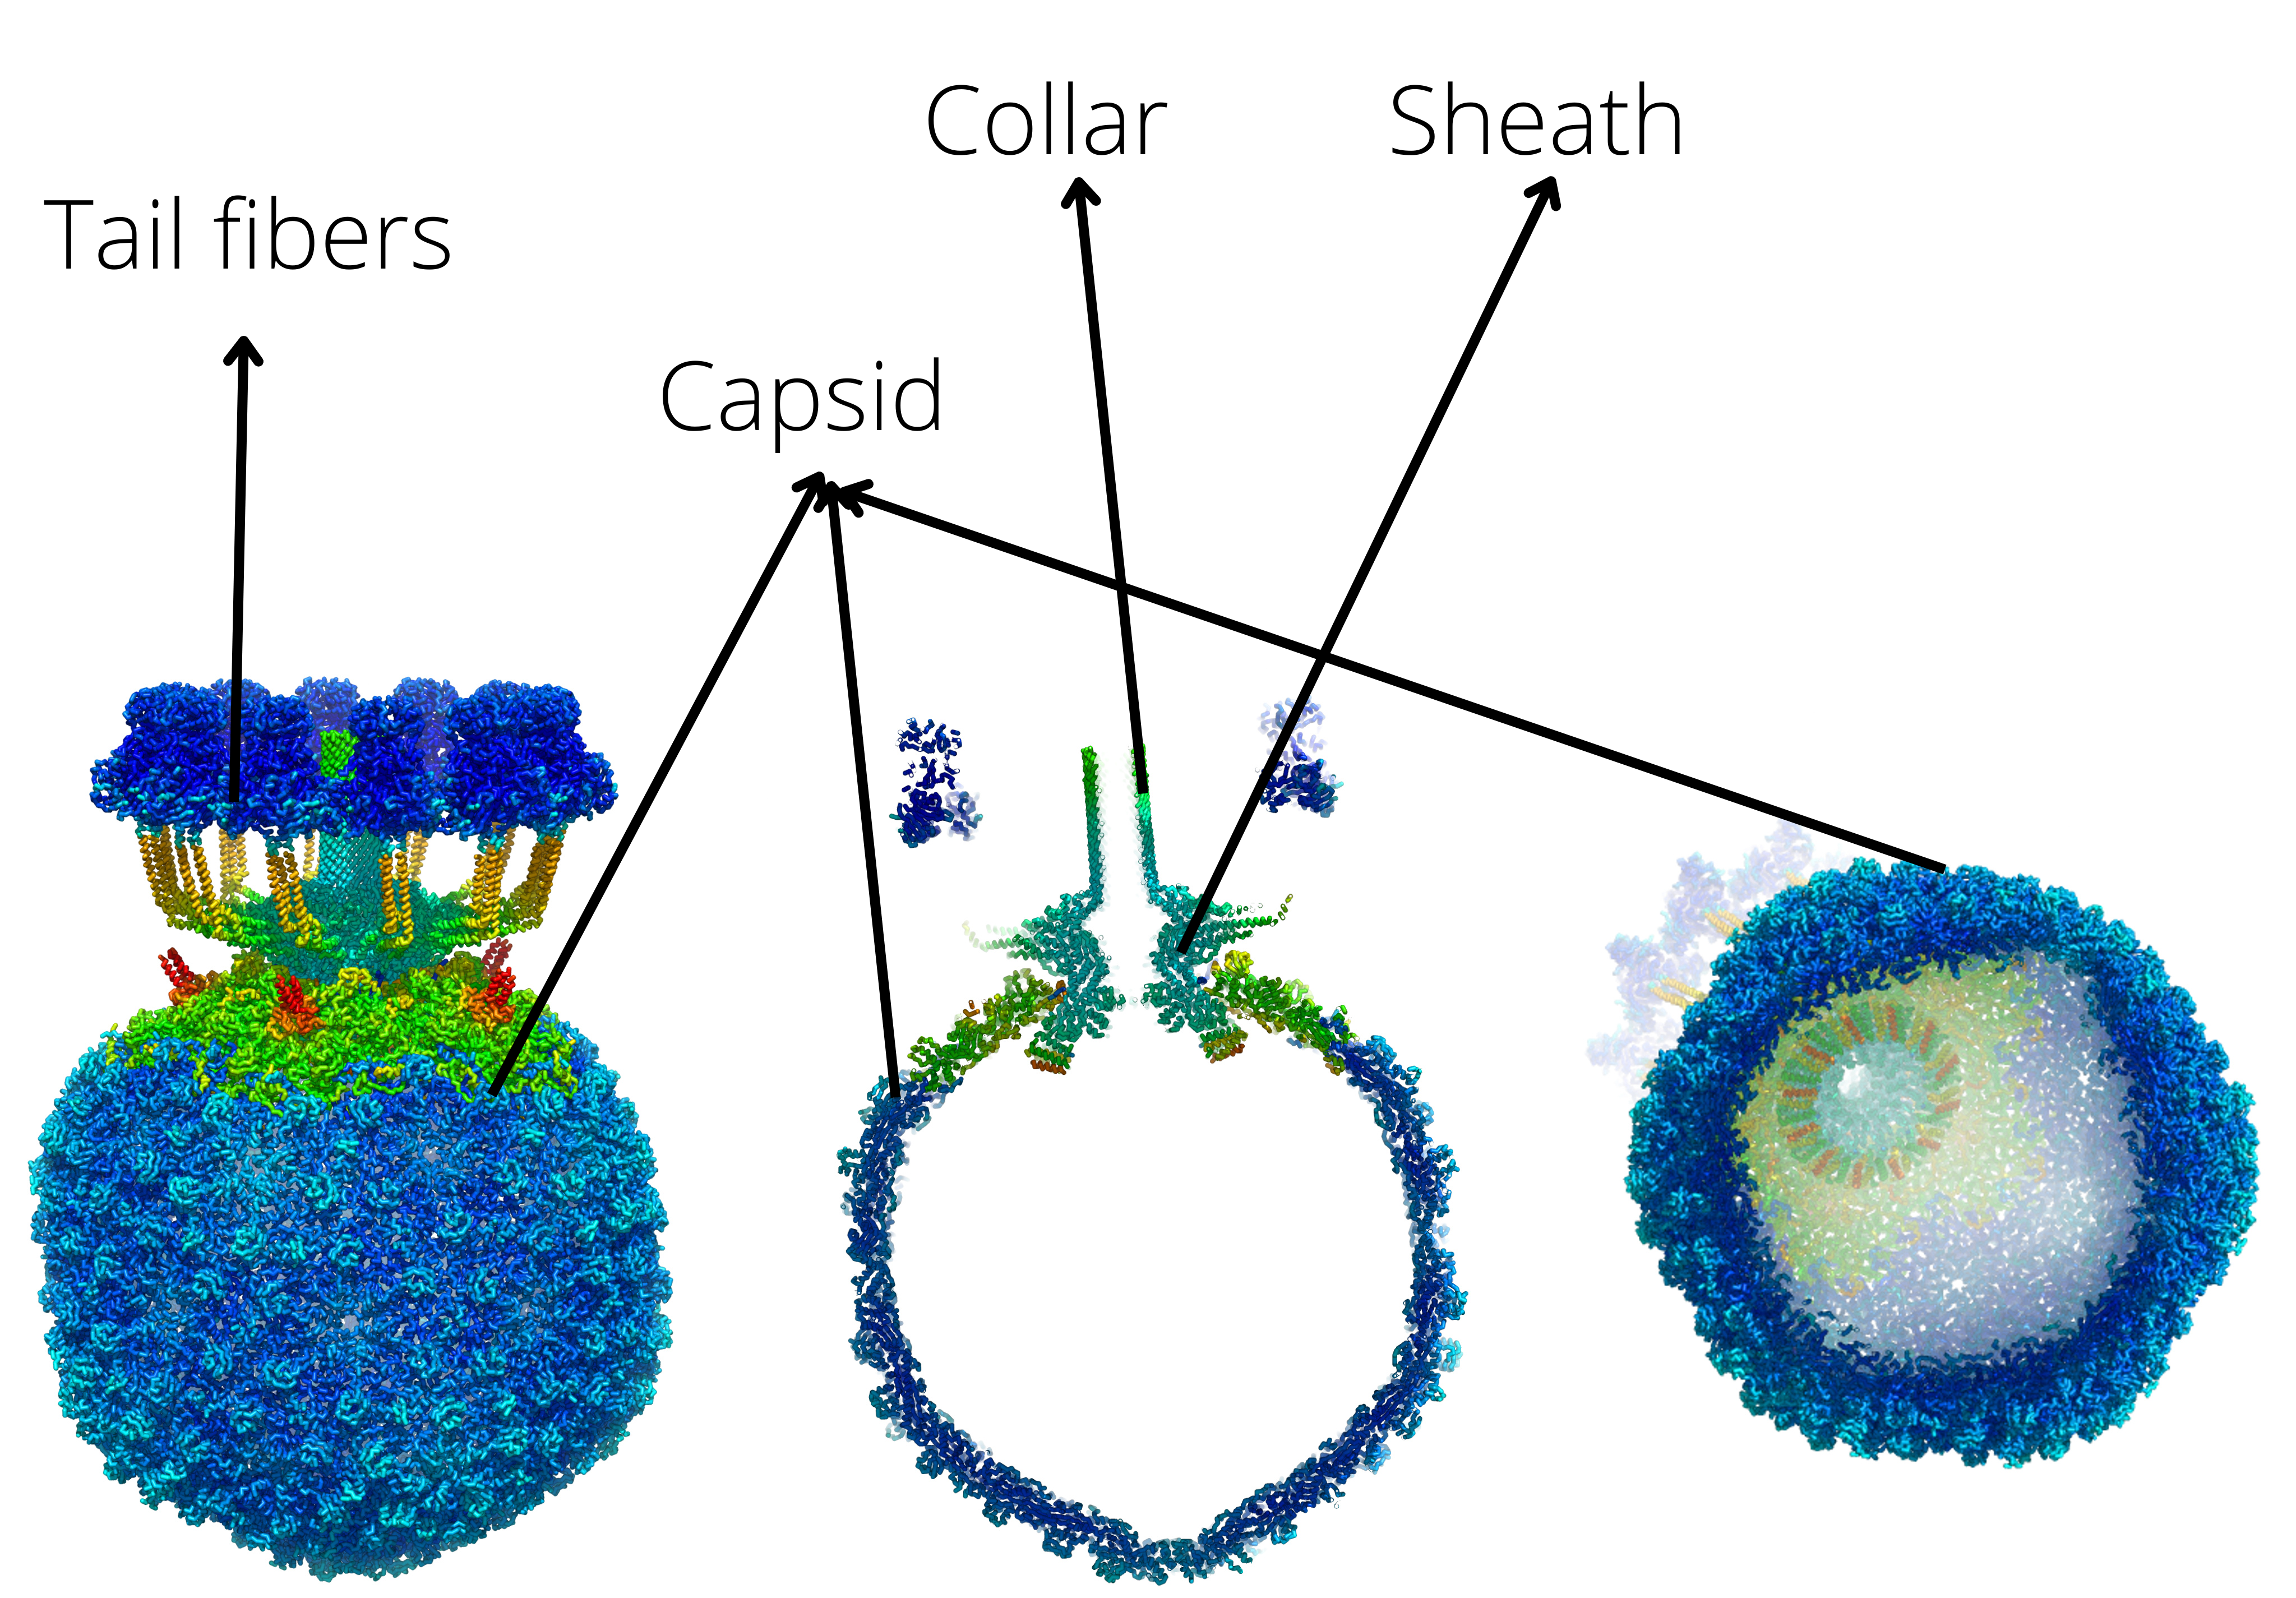
\includegraphics[width=0.90\textwidth]{p68.png}\end{figure}\end{center}
These three views allow us to see the capsid, the collar, and sheath, the tail fibres, and the spikes, which are integrated into the collar. The tail fibres act exactly like the Coronavirus spike proteins: they bind to a specific compound on the surface of the bacteria, but they don't access it. They only bind to the surface, perforate it using the spikes and then, due to a difference in pressures, the genetic material is injected into the cell. Then, it uses the fact that bacteria will integrate strands of genetic material floating in the environment into its own hereditary material in order to force the host to reproduce the virus.
\paragraph{}Using the PDB2STL pymol\footnote{Pymol: program that takes a protein database and converts it into a viewable model} tool, I managed to create a printable 3D model of the virus, which was then polished using a wire brush and painted gray so the details can be seen with more clarity. Then, a white filament strand was added to symbolize the genetic material being oozed into a cell:
\begin{center}\begin{figure}[H]\centering\includegraphics[width=0.50\textwidth]{3dirl.jpg}\end{figure}\end{center}

% > > > Theorem Environments
%----------------------------------------------------------------------------------------------------------------------------------------------------------%
\chapter{Conclusions}
%----------------------------------------------------------------------------------------------------------------------------------------------------------%
\section{Experimental conclusions}
This study has concluded that the prevalence of \emph{Staphylococcus Aureus} in our high school is 48,8\%, a 150\% of the percentage expected. As explored previously, this could mostly be due to climate change or antibiotic abuse.
%----------------------------------------------------------------------------------------------------------------------------------------------------------%
\section{Bibliographic conclusions}
(is this even needed?)
%----------------------------------------------------------------------------------------------------------------------------------------------------------%
\section{Strengths and weakneses}
This research was not without its strengths, but neither was it without its weakneses.
\paragraph{Strengths} The protocol was adapted fairly well to the environment it was run in, and no incidents took place during the realisation of the experimentation.
\paragraph{Weakneses} While the Agar plates used were definitely adequate for the purpose they were used for, a much more appropriate growth medium called Baird-Parker (BP) could've been used.
% > > > Works Cited
%\include{chapters/chapter05}
% > > > What is LaTeX
%\include{chapters/chapter06}
%----------------------------------------------------------------------------------------------------------------------------------------------------------%
\backmatter
\renewcommand{\thepage}{\Roman{page}}\setcounter{page}{0}
\clearpage
\printbibliography[title={Works referenced}]
\part{Appendix}\appendix
\chapter{Annex 1 – Informed consent given to subjects before sampling}
\includepdf[pages=-]{consent.pdf}
\clearpage\appendix\chapter{Annex 2 – GDPR notice given to subjects before sampling}
\includepdf[pages=-]{gdpr.pdf}
\chapter{Annex 3 – Protocol as published in protocols.io}
\includepdf[pages=-]{protocol.pdf}
\chapter{Annex 4 – Bibliography consulted}
\includepdf[pages=4-last]{refs.pdf}
\end{document}
